\label{chap:background}

There are different types optimizations that can be performed on a program to improve its
performance. The optimization can be made for finding data locality and hence extracting
parallelism. Starting from the early history of programming languages the internal representation
of program is done with Abstract Syntax Tree(AST). Though some elementary transformation can
be performed on AST it is tough to carry out complex transformations like dependency analysis among
statements inside a loop. Trees are very rigid data structures to do such transformations.
In this chapter an extremely powerful mathematical model which puts together analysis power,expressiveness and flexibility is explained in detail.

\section{Program transformations with polyhedral model}

In this section some of the common program transformations which can be realized with the
assistance of polyhedral model are explained. The polyhedral model is not a normal
representation of programs when compared to the
classical structure of programs(like AST) that every programmer is familiar with. But
it is easier to do transformations smoothly in this model.

\subsection{Transformation for improving data locality}

The polyhedral model can detect common array accesses which improves the data locality. It is
illustrated with a simple example.
{\footnotesize
\begin{lstlisting}
  for(i = 1; i <= 10; i++)
    A[i] = 10;

  for(j = 6; j <= 15; j++)
    A[j] = 15;
\end{lstlisting}
}

The two loops will be represented by two polyhedrons and it can find the common 
array accesses starting from index 6 to 10 and the code can be transformed as follows.

{\footnotesize
\begin{lstlisting}
for(i = 1; i <= 5; i++)
  A[i] = 10;
for(j = 6; j <= 15; j++)
  A[j] = 15;
\end{lstlisting}
}

\subsection{Scalar expansion}
{\footnotesize
\begin{lstlisting}
for (i = 0; i < 8; i++)
  sum += A[i];
\end{lstlisting}
}
With the support of memory access transformation in polyhedral model this loop
can be executed in parallel. It can be transformed to the code below where the scalar 'sum'
is changed to array 'tmp'.  
{\footnotesize
\begin{lstlisting}
<create and initialize an array 'tmp' with size 4>
for (i = 0; i < 8; i++)
   tmp[i % 4] += A[i];
sum = tmp[0] + tmp[1] + tmp[2] + tmp[3];
\end{lstlisting}
}
With the help of some optimizer (like PLUTO\cite{pluto}) the following code
can be generated, where the outer loop is parallel.
{\footnotesize
\begin{lstlisting}
parfor (ii = 0; ii < 4; ii++)
  tmp[ii] = 0;
  for (i = ii * 2; i < (ii+1) * 2; i++)
    tmp[ii] += A[i];
sum = tmp[0] + tmp[1] + tmp[2] + tmp[3];
\end{lstlisting}
}
%\subsection{Constant propagation through arrays}
%\subsection{Eliminate dead loop iterations}
%\subsection{Automatic parallelization}
%\subsection{Vectorization}

\section{Polyhedral representation of programs}

The polyhedral model does its transformations based on linear algebra and linear programming.
Certain parts of programs known as SCoPs(Static Control Part) are represented in this model.
A program part that can be represented using polyhedral model is called SCoPs. Generally
loops are the candidates for SCoPs. There are some restrictions to the set of statements 
in the section of code to be qualified as SCoP. Those are listed below.

\begin{itemize}
\item The set of statements in the loops should have bounds and conditionals having affine functions(linear
combination with constant) of surrounding iterators and the parameters (constants whose values are unknown at compile time).
\item There should be structured control flow.
\item Side effect free(Only pure functions are allowed)
\end{itemize}

There are efforts to increase the application domain of polyhedral model \cite{Benabderrahmane}
which shows most of the restrictions are artificial.

The representation of polyhedral model has three parts. Each of them is explained in detail with simple
examples in the following sections.

\subsection{Iteration domain}
Consider the following loop.
{\footnotesize
\begin{lstlisting}
for (int i = 2; i <= N; i++)
  for (int j = 2; j <= N; j++)
    A[i] = 10; // S1
\end{lstlisting}
}
Notice that the statement A[i] = 10 is denoted by S1. Even though this is a single statement, considering
the loop as a whole it has several statement instances along the life time of the loop. Each statement
instance has an \textbf{iteration vector} associated with it. In general the iteration vector for S1 is (i,j).
To be more precise each statement instance has its own iteration vector. The set of all iteration vectors
for a given statement is called \textbf{iteration domain} of that statement. Since the value of N
is not known at compile time and the value is unchanged while runtime we call N as \textbf{parameter}.
Hence the above loop is \textbf{parametric}. For the above loop we can write the iteration domain mathematically as
\begin{center}
$D_{S1}\ =\ \{(i,j)\ \epsilon\ Z^2\ |\ 2\ \leq\ i\ \leq\ N\ \wedge\ 2\ \leq\ j\ \leq\ N\}$
\end{center}
This is a subspace of $Z^2$. To get a better view this can be represented graphically as in Figure ~\ref{fig:iter}
\begin{figure}
\begin{center}
  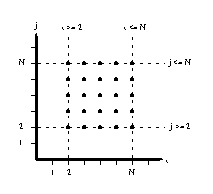
\includegraphics[height=8cm,width=8cm]{images/iter.eps}
  \caption{Graphical representation of iteration domain(S1)}
  \label{fig:iter}
\end{center}  
\end{figure}

\noindent
Consider another example by just adding a conditional statement
{\footnotesize
\begin{lstlisting}
for (int i = 2; i <= 6; i++)
  for (int j = 2; j <= 6; j++)
    if(i <= j)
      A[i] = 10; // S2
\end{lstlisting}
}
\noindent
And the iteration domain here is as below and the corresponding graphical representation is shown in Figure ~\ref{fig:iter1}

\begin{center}
$D_{S2}\ =\ \{(i,j)\ \epsilon\ Z^2\ |\ 2\ \leq\ i\ \leq\ 6\ \wedge\ 2\ \leq\ j\ \leq\ 6\ \wedge\ i\ \leq\ j\}$
\end{center}
\begin{figure}
\begin{center}
  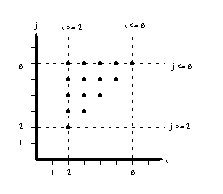
\includegraphics[height=8cm,width=8cm]{images/iter1.eps}
  \caption{Graphical representation of iteration domain(S2)}
  \label{fig:iter1}
\end{center}  
\end{figure}

It can be seen that the iteration domain is specified by set of constraints. When those constraints are
affine and depend only on the outer loop induction variables and parameters, the set of constraints
defines a polyhedron (Z-polyhedron, polyhedron for short). Hence it has got the name Polyhedral Model.

\subsection{Schedule}

The iteration domain does not give any information on the order of statements to be executed. If there
is no order specified among the execution of statements it means that all the statements can be executed
in parallel. But due to data dependences this assumption may not be always true. So a method is devised
to represent this order of execution which is called \textbf{scattering} function. There are many
kinds of scattering in polyhedral model, as allocation, scheduling, chunking. For simplicity
we are dealing only with \textbf{scheduling}. We are free to select any scheduling for better
transformation and hence better parallelism.
Consider the following loop.
{\footnotesize
\begin{lstlisting}
for (int i = 2; i <= 4; i++)
  for (int j = 2; j <= 4; j++)
    P[i][j] = A[i] * B[j] ; // S3
\end{lstlisting}
}
\noindent
We can define a scheduling(scattering) function:
\begin{center}
$\phi_{S3}(i,j) = (i,j)$
\end{center}, which means that each iteration vector (i,j) in the iteration domain is associated with
a logical date. That is the statement instances need to be executed in the lexicographical order of the
logical date. Another possible scattering function would be:
\begin{center}
$\phi_{S3}(i,j) = (j,i)$
\end{center}
\noindent
It is possible to generate code for the changed schedule with ClooG\cite{cloog}. The
transformed code is:
{\footnotesize
\begin{lstlisting}
for (t1 = 2; t1 <= 4; t1++) {
  for (t2 = 2; t2 <= 4; t2++) {
    i = t2; j = t1;
    P[i+j] += A[i] + B[j];
  }
}
\end{lstlisting}
}
\noindent
It can be observed that we just performed loop interchange.
\subsection{Access function}
Consider a statement with array access A[i+j][i+N]. The \textbf{access function} corresponding to this can be written
as:
\begin{center}
$F_A(i,j) = (i+j,i+N)$
\end{center}
We can manipulate the access function for achieving better data locality and parallelism.

In general any optimization framework which makes use of polyhedral model will
transform the code through the blocks shown in Figure ~\ref{fig:poly_steps}.
As the first stage dependence analysis is carried out followed by representing
it by polyhedral model in terms of iteration domain, schedule and access function.
This is further transformed for better optimization and code is generated
for this.
\begin{figure}
  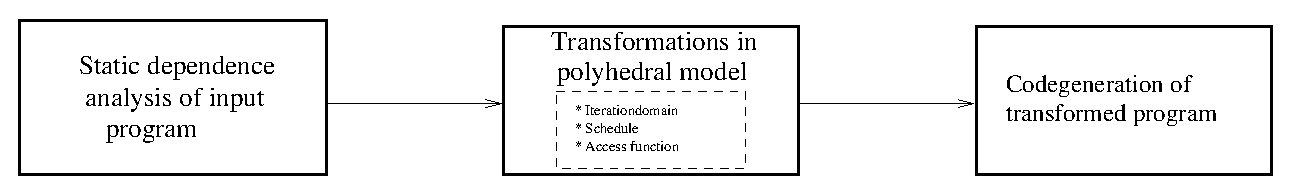
\includegraphics[width=1\textwidth]{images/poly_steps.eps}
  \caption{Transformation in polyhedral model}
  \label{fig:poly_steps}
\end{figure}
